\section{Conclusions and perspectives}
\subsection{Results summary}
\begin{itemize}
    \item The Kalman filter has not been proven interesting enough for post-processing day-ahead irradiance forecasts, in opposition to what was said in \cite{suksamosorn_post-processing_2021} paper. The difference may be due to the fact that we used a more precise GFS data in comparison to the WRF data used in the paper. What is more, I dealed with the extreme case of day-ahead data with origin 00:00 UTC, while the paper fixed the origin at 13:00 (local hour).

    A more appropriate use of the Kalman filter would be for filtering faulty data, as explored in \cite{sec:filtering}.
    \item For a MAE minimisation, the SVR model clearly yielded the best results, both for post-processing a single NWP model and for hybridation. This confirms \cite{verbois_statistical_2022}.
    \item For a RMSE minimisation, there is no clear consensus for post-processing a single NWP model, as it was the case in the literature where the random forest (\cite{suksamosorn_post-processing_2021}), GBM and MLP models (\cite{verbois_statistical_2022}) were deemed promising. Still the MLP model as well as the linear least square regression model stand out.

    The hybridation showed some limits of the MLP model, in favor of the linear model.
    \item Using the LT CONT model on post-processed data only yielded marginal enhancements in metrics, whereas using the adequate model (SVR for MAE, Linear regression for RMSE) on the whole dataset provided significant improvements as compared to the LT CONT model.
\end{itemize}

\subsection{Perspectives}
\begin{itemize}
    \item The specific study case was the one of the day-ahead irradiance forecasts, but such models can be applied to any other timestamped variable.
    \item Many improvements and fine-tuning can be performed on the actual model. All of them are listed in the README of my project \cite{myrepo}.
    \item There are also more advanced promising models that could be investigated, also listed in the README. Among them, one can mention the N-BEATS models and the Meta-Transformer model depicted in \autoref{fig:innovative_models}.
\end{itemize}

\begin{figure}[htb!]
    \begin{subfigure}[h]{0.4\linewidth}
        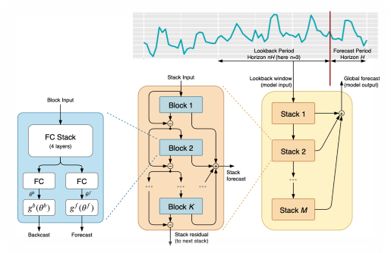
\includegraphics[width=\columnwidth]{figures/n-beats.png}
        \caption{N-BEATS architecture.}
        \source{\cite{oreshkin2020nbeats}}
    \end{subfigure}
    \hfill
    \begin{subfigure}[h]{0.4\linewidth}
        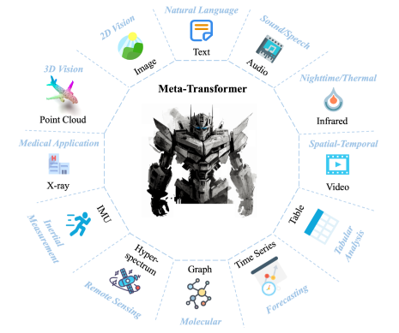
\includegraphics[width=\columnwidth]{figures/meta-transformer.png}
        \caption{Meta-Transformer.}
        \source{\cite{zhang2023metatransformer}}
    \end{subfigure}
    \caption{Two innovative models for post-processing timestamped variables.}
    \label{fig:innovative_models}
\end{figure}
\subsection{My learnings from the internship}